\documentclass[10pt,svgnames,usenames,table]{beamer} %,handout si version papier
\NeedsTeXFormat{LaTeX2e} 

\usetheme[compress]{Singapore} % theme

\usepackage[french]{babel}
\usepackage[utf8x]{inputenc} % pour les accents (mettre latin1 pour
                            % windows au lieu de utf8)
\usepackage[T1]{fontenc}
\usepackage{amsmath,amsthm,amssymb}        % un packages mathématiques
\usepackage{xcolor}         % pour définir plus de couleurs
\usepackage{graphicx}       % pour insérer des figures
\usepackage{lmodern}
\usepackage{url}
	\urlstyle{sf}
\usepackage{lastpage}
\usepackage{endnotes}
\usepackage{listings}
\usepackage[french]{varioref}
\usepackage{wrapfig}
\usepackage{pdfpages}
\usepackage{verbatim}
\usepackage{graphicx}

%\usepackage[svgnames]{color}
%\definecolor{webdarkblue}{rgb}{0,0,0.4}
%\definecolor{webgreen}{rgb}{0,0.3,0}
%\definecolor{webblue}{rgb}{0,0,0.8}

\setbeamercolor{section in head/foot}{use=structure,bg=structure.fg!25!bg} % "Amélioration du jeu de couleur"
%\useoutertheme[subsection=true]{smoothbars} % Pour avoir un rappel de la subsection
\setbeamerfont{frametitle}{series=\bfseries}
\setbeamertemplate{frametitle}[default][center] % Titre centré et bien placé.


% "Fioriture de style" : qd <x-> dans les item, les autres en gris clair
\beamertemplatetransparentcovered


% Comportement des itemize
\setbeamertemplate{itemize item}[ball]
\setbeamertemplate{itemize subitem}[triangle]
\setbeamertemplate{itemize subsubitem}[circle]

%\renewcommand\sfdefault{cmss} % Polices

% Les block arrondis et ombrés dans la couleur que je veux
\setbeamertemplate{blocks}[rounded][shadow=true]
\definecolor{normalBlockColor}{RGB}{102,153,255}
\definecolor{normalTitleBlockColor}{RGB}{0,0,102}
\definecolor{normalBlockTextColor}{RGB}{255,255,255}
\definecolor{normalBlockTitleTextColor}{RGB}{255,255,255}
\definecolor{exampleBlockColor}{RGB}{202,251,197}
\definecolor{exampleTitleBlockColor}{RGB}{166,241,158}
\definecolor{exampleBlockTextColor}{RGB}{0,0,0}
\definecolor{exampleBlockTitleTextColor}{RGB}{0,120,0}
\definecolor{alertBlockColor}{RGB}{248,218,218}
\definecolor{alertTitleBlockColor}{RGB}{244,108,108}
\definecolor{alertBlockTextColor}{RGB}{0,0,0}
\definecolor{alertBlockTitleTextColor}{RGB}{120,0,0}
\setbeamercolor*{block title}{fg=normalBlockTitleTextColor,bg=normalTitleBlockColor}
\setbeamercolor*{block body}{fg=normalBlockTextColor,bg=normalBlockColor}
\setbeamercolor*{block title alerted}{fg=alertBlockTitleTextColor,bg=alertTitleBlockColor}
\setbeamercolor*{block body alerted}{fg=alertBlockTextColor,bg=alertBlockColor}
\setbeamercolor*{block title example}{fg=exampleBlockTitleTextColor,bg=exampleTitleBlockColor}
\setbeamercolor*{block body example}{fg=exampleBlockTextColor,bg=exampleBlockColor}
\setbeamerfont{block title}{size={}}



%------------ fin style beamer -------------------

% Faire apparaître un sommaire avant chaque section
% \AtBeginSection[]{
%   \begin{frame}
%   \frametitle{Plan}
%   \medskip
%   %%% affiche en début de chaque section, les noms de sections et
%   %%% noms de sous-sections de la section en cours.
%   \small \tableofcontents[currentsection, hideothersubsections]
%   \end{frame} 
% }


% Pour personnaliser la barre de navigation du dessous
\setbeamertemplate{navigation symbols}{
	%\insertslidenavigationsymbol
	%\insertframenavigationsymbol
	%\insertsubsectionnavigationsymbol
	\quad\textbf{\insertframenumber/\inserttotalframenumber} % Numéro de page
	%\insertsectionnavigationsymbol
	%\insertdocnavigationsymbol
	%\insertbackfindforwardnavigationsymbol
}
% Supprimer les icones de navigation (pour les transparents)
%\setbeamertemplate{navigation symbols}{}

% Mettre les icones de navigation en mode vertical (pour projection)
% \setbeamertemplate{navigation symbols}[vertical]

\newenvironment{itemize2}%
	{ \begin{list}%
		{$\bullet$}%
		{\setlength{\labelwidth}{30pt}%
		 \setlength{\leftmargin}{35pt}%
		 \setlength{\itemsep}{\parsep}}}%    
	{ \end{list} }

\def\siecle#1{\textsc{\romannumeral #1}\textsuperscript{e}~siècle} % => le \siecle{19}

\definecolor{codeBlue}{rgb}{0,0,1}
\definecolor{webred}{rgb}{0.5,0,0}
\definecolor{codeGreen}{rgb}{0,0.5,0}
\definecolor{codeGrey}{rgb}{0.6,0.6,0.6}
\definecolor{webdarkblue}{rgb}{0,0,0.4}
\definecolor{webgreen}{rgb}{0,0.3,0}
\definecolor{webblue}{rgb}{0,0,0.8}
\definecolor{orange}{rgb}{0.7,0.1,0.1}
\lstset{
      language=C,
      flexiblecolumns=true,
      numbers=left,
      stepnumber=1,
      numberstyle=\ttfamily\tiny,
      keywordstyle=\ttfamily\textcolor{blue},
      stringstyle=\ttfamily\textcolor{red},
      commentstyle=\ttfamily\textcolor{green},
      breaklines=true,
      extendedchars=true,
      basicstyle=\ttfamily\scriptsize,
      showstringspaces=false
    }

\usepackage{pdflscape} %% portrait
\usepackage[french]{varioref} % \vpageref
\usepackage{pgfplots}

\newcommand{\badet}{et}
\newcommand{\goodet}{\mathbin{\mathrm{et}}}

\graphicspath{{img/}}
\definecolor{gris}{RGB}{228,228,228}
\definecolor{bleu}{RGB}{34,148,255}
\definecolor{darkgray}{rgb}{0.3,0.3,0.3}

\usefonttheme[onlymath]{serif} % to see the difference when I do mathsf

\logo{
\includegraphics[height=5mm]{logo_12-13-mini.png}}
\institute{Louvain-li-Nux}
\title{\textbf{Formation \LaTeX}\\
Introduction à l'écriture de document \textrm{\LaTeX}}
\author{Arnaud \textsc{Cerckel} \and Benoît \textsc{Legat}}

%\date{24 mars 2015}


% A changer (selon Arnaud) le utf8x pas aligné slide 12/30
% maketitle
%
%
\begin{document}

%%%%%%%%%%%% SIDA
\begin{landscape}
\begin{frame}[noframenumbering,plain]
	\vspace{-.5cm}
	\hspace*{.1mm}
	
\includegraphics[page=1,height=\paperwidth]{latex_sida.pdf}
\end{frame}
\end{landscape}
%%%%%%%%%%%%

\begin{frame}
\maketitle
Merci à Jolan \textsc{Wolter} et Thomas \textsc{Vanzieleghem} pour avoir réalisé la première version de ces slides
ainsi qu'à David \textsc{Ernst} et Matthieu \textsc{Baerts} pour avoir réalisé la deuxième version.
\end{frame}

\AtBeginSection[]
  {
     \begin{frame}<beamer>
     \frametitle{\insertsection}
     \tableofcontents[hideothersubsections]
     \end{frame}
  }

\section{Introduction}
\subsection{Qu'est-ce que \LaTeX{}?}
\begin{frame}
\frametitle{Qu'est ce que \LaTeX}

\begin{itemize}
\item \TeX{} $ \Rightarrow$ programme de mise en page
\vspace{0.5cm}
\item \LaTeX{} $ \Rightarrow$ ensemble de commandes qui seront
 interprétées par le programme \TeX
 \vspace{0.5cm}
\item \LaTeX{} $ \neq$ WYSIWYG (What You See Is What You Get)
\end{itemize}

\end{frame}

\begin{frame}{Premier angle de comparaison}
  \begin{description}
    \item[Auteur]
      %\begin{center}
      \begin{tabular}{|lll|}
        %\hline
        %& Créateur & Description du créateur\\% selon wikipédia\\
        \hline
        Office & Microsoft & No comment\\
        %Microsoft Word & Microsoft & Microsoft used monopolistic business practices and anti-competitive strategies including refusal to deal and tying, put unreasonable restrictions in the use of its software, and used misrepresentative marketing tactics; both the U.S. Department of Justice and European Commission found the company in violation of antitrust laws\\
        \TeX & Donald Knuth & Père de l'algorithmie\\
        \hline
      \end{tabular}
      %\end{center}
    \item[But]
      \begin{tabular}{|lp{0.5\textwidth}|}
        \hline
        %Soft & Créateur & Description du créateur\\% selon wikipédia\\
        %Office & Microsoft & No comment\\
        %Microsoft Word & Microsoft & Microsoft used monopolistic business practices and anti-competitive strategies including refusal to deal and tying, put unreasonable restrictions in the use of its software, and used misrepresentative marketing tactics; both the U.S. Department of Justice and European Commission found the company in violation of antitrust laws\\
        Office & Être utilisable par n'importe qui sans connaissance ni
        formation particulière pour aider à ancrer le monopole de Microsoft
        grâce aux formats propriétaires \texttt{.doc}, \texttt{.xls}, \dots\\
        \TeX & Améliorer sa productivité et
        la qualité de rendu de ses documents sur l'algorithmie\\
        \hline
      \end{tabular}
    \item[Licence]
      \begin{tabular}{|lp{0.5\textwidth}|}
        %\hline
        %& Créateur & Description du créateur\\% selon wikipédia\\
        \hline
        Office & Propriétaire jusqu'au format (incompatibilité
        voulue par Microsoft)\\
        %Microsoft Word & Microsoft & Microsoft used monopolistic business practices and anti-competitive strategies including refusal to deal and tying, put unreasonable restrictions in the use of its software, and used misrepresentative marketing tactics; both the U.S. Department of Justice and European Commission found the company in violation of antitrust laws\\
        \TeX & Libre et open source\\
        \hline
      \end{tabular}
  \end{description}
\end{frame}


\subsection{Pourquoi \LaTeX{}?}
\begin{frame}{Pourquoi \LaTeX{}?}

  \begin{itemize}
  	\item Qualité professionnelle de document
	\item Facilité d'emploi des :
	\begin{itemize}
		\item formules mathématiques
		\item table des matières
		\item références bibliographiques
		\item références croisées
		\item ...
	\end{itemize}
	\item Séparation entre contenu et forme
	\item Description du contenu indépendant de la forme
	\item Gratuit
	\item Stable, même pour les très gros documents
  \end{itemize}
\end{frame}

\begin{frame}{Pourquoi \LaTeX{}?}

\begin{figure}[htbp]
\begin{center}
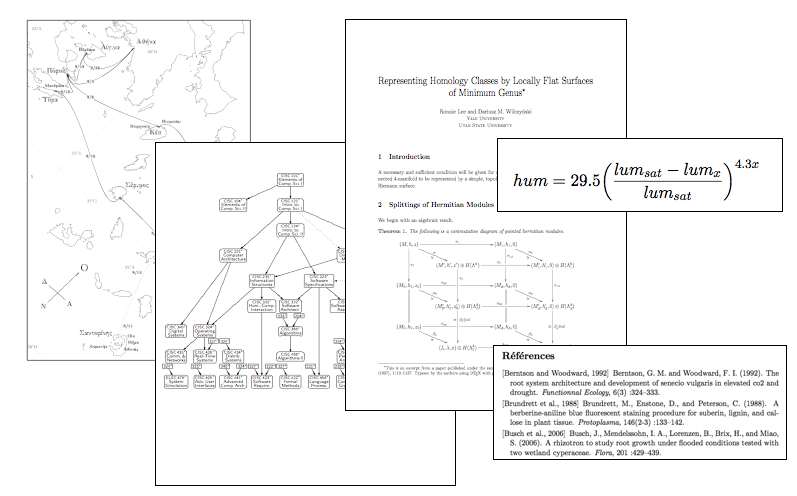
\includegraphics[height=6.5cm]{latex_exemples}
\end{center}
\end{figure}
\end{frame}

%-----------------------
\subsection{Pourquoi pas \LaTeX{}?}
\begin{frame}{Pourquoi pas \LaTeX{}?}

  \begin{itemize}
  	\item Les tableaux...
	\item Prise en main plus longue que pour traitement de texte WYSIWYG
	\item Je suis allergique à toute forme de code informatique
	\item J'ai des actions Microsoft
	\item Je ne trouve pas le ``\textbackslash'' sur mon clavier
  \end{itemize}
\end{frame}

\begin{frame}{Oui mais...}
  \begin{center}
    %\resizebox{\textwidth}{!}{
    \begin{tikzpicture}
      \begin{axis}[xmin=0, xmax=4, ymin=-2, ymax=5,
          xlabel={Expérience, maitrise}, ylabel=Productivité,
        legend style={at={(0.01,0.99)}, anchor=north west}]
        \addplot[smooth, color=blue]{x-0.05};
        \addlegendentry{\LaTeX}
        \addplot[smooth, color=red,domain=0:5]{sqrt(x)};
        \addlegendentry{Word}
        %\xlabel{Productivité}
        %\ylabel{Expérience/maitrise}
      \end{axis}
      \foreach \x/\com/\deltax/\deltay/\adj in {
        {1.1}/{Maintenant}/{0}/{0.8}/below,
        {2.2}/{Après la formation}/{0}/{0.4}/below,
        {4.6}/{À l'heure de votre mémoire}/{0}/{1.2}/below
      } {
        %\fill \coord circle (100pt) node[\adj] {$\coord$};
        \draw[dashed] (\x,0) -- (\x+\deltax,\deltay) node[above] {\com};
        %\draw (\x+\deltax,\deltay) node {\com};
      }
    \end{tikzpicture}
    %}
  \end{center}
\end{frame}

%-----------------------
\subsection{Les Outils}
\begin{frame}{Ce qu'il faut pour commencer.}

  \begin{itemize}
	  \item GNU/Linux
	  \begin{itemize}
	  	\item Distribution \LaTeX{} = \textbf{TeXLive}
		\item Éditeur de texte = \textbf{TeXMaker, LaTeXila, Kile}
	  \end{itemize}
	  \item Windows
	  \begin{itemize}
	  	\item Distribution \LaTeX{} = \textbf{MikTeX}
		\item Éditeur de texte = \textbf{TeXMaker, TeXnicCenter}
	  \end{itemize}
	  \item Mac OS
	  \begin{itemize}
	  	\item Distribution \LaTeX{} = \textbf{MacTeX}
		\item Éditeur de texte =\textbf{TeXMaker, TeXShop, iTeXMac}
	  \end{itemize}
  \end{itemize}
\end{frame}

\section{Les concepts de base}
\subsection{Les fichiers}

\begin{frame}{Les fichiers}

	\begin{center}
		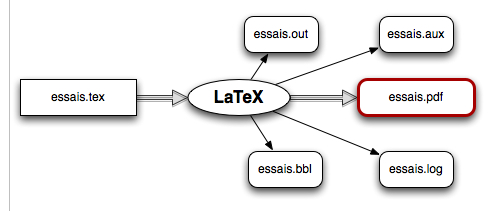
\includegraphics[height=3cm]{compilation.jpg}
	\end{center}

	\begin{itemize}
		\item Fichier source  = essais\alert{\textbf{.tex}}
		\item Lors de compilation $\rightarrow$ création de nombreux fichiers annexes
		\begin{itemize}
			\item style, class;
			\item structure du document;
			\item table des matières, liste des figures;
			\item liste des références;
			\item ...
		\end{itemize}
		\item Création d'un fichier essais\alert{\textbf{.pdf}}
	\end{itemize}
\end{frame}

\begin{frame}[fragile]
  \frametitle{Encoding}
  \begin{columns}
    \begin{column}{0.5\textwidth}
      \begin{itemize}
        \item En anglais, ASCII est suffisant, 1 byte par caractère;
        \item UTF-8, 1 byte pour un caractère simple, plus de bytes pour un plus exotique;
        \item latin-1, \dots, à éviter.
        \item Les caractères ASCII sont les mêmes pour tous les encodages !
        \item Si vous en utilisez d'autres (e.g. accent), \LaTeX{} doit savoir l'encodage !
        \item Le package \lstinline|inputenc| (INPUT ENCoding) s'en charge !
      \end{itemize}
    \end{column}
    \begin{column}{0.5\textwidth}
      \centering
      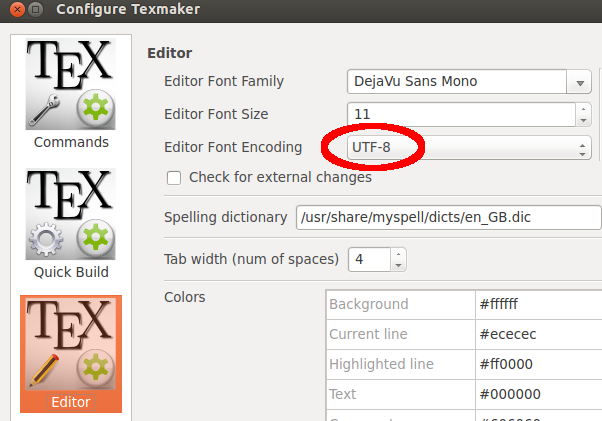
\includegraphics[width=\linewidth]{img/utf8_circle.png}
    \end{column}
  \end{columns}
\end{frame}

%-----------------------
\subsection{La structure}

\begin{frame}[fragile]{Structure générale du document}
\framesubtitle{Séparation du préambule et du corps du document}
\small
\begin{tabular}{ll}
  Type de document &
  \lstinline|\documentclass[a4paper, 10pt]{article}|\\
  Utilisation de \textit{package} &
  \lstinline|\usepackage[utf8x]{inputenc} % ou [utf8]|\\
  Utilisation de \textit{package} &
  \lstinline|\usepackage[T1]{fontenc}|\\
  Utilisation de \textit{package} &
  \lstinline|\usepackage[french]{babel}|\\
  Utilisation de \textit{package} &
  \lstinline|\usepackage{lmodern}|\\
  Blanc pour la lisibilité &\\
  Début du document &
  \lstinline|\begin{document}|\\
  Corps du document &
  \lstinline|Ceci est mon premier document en \LaTeX{}|\\
  Fin du document &
  \lstinline|\end{document}|\\
\end{tabular}


\end{frame}

%-----------------------

\subsection{Les classes}

\begin{frame}[fragile]{Les principales classes de document}
\begin{tabular}{lp{8cm}}
  \textbf{article} & pour les articles de journaux scientifiques, présentations, rapports courts...\\
  \textbf{report} & pour de plus long rapports de plusieurs chapitres, petits livres, thèses, ...\\
  \textbf{book} & pour de vrais livres.\\
  \textbf{letter} & pour écrire des lettres.\\
  \textbf{beamer} & pour écrire des présentations (comme celle-ci).
\end{tabular}
\vspace{1cm}
\begin{center}
\verb|\documentclass[a4paper,10pt]{article}|\\
\end{center}
\end{frame}

\subsection{La structure}
\begin{frame}[fragile]{La structure logique du document}
	\begin{itemize}
		\item Structure logique du document uniquement
		\item \LaTeX{} se charge de la numérotation et de la mise en page\\
	\end{itemize}
	\vspace{1cm}

	\verb|\part{}|\\
	\hspace{1cm} \verb|\chapter{}| \hspace{2cm}$\Longrightarrow$ \textcolor{bleu}{uniquement \textit{books}}\\
	\hspace{2cm} \verb|\section{}|\\
	\hspace{3cm} \verb|\subsection{}| \\
	\hspace{4cm} \verb|\subsubsection{}| \\
	\hspace{5cm} \verb|\paragraph{}	| \\

\end{frame}

%-----------------------
\section{Mise en page générale}
\subsection{La table des matières}
\begin{frame}[fragile]{Table des matières}
	\begin{itemize}
		\item Une ligne de commande suffit pour générer toute la table des matières
	\end{itemize}
	\begin{columns}
      \begin{column}{0.5\textwidth}
        \begin{lstlisting}
\begin{document}
\tableofcontents
\section{Introduction}
Ceci est mon premier document en \TeX{}
\section{Le vif du sujet}
Le sujet est en or mais pas le vif.
\subsection{Mais quel est le sujet ?}
\LaTeX{}, ce logiciel d'exception !
\end{document}
        \end{lstlisting}
      \end{column}
      \begin{column}{0.5\textwidth}
        \begin{flushright}
          \fbox{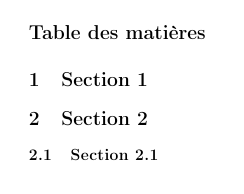
\includegraphics[width=0.6\textwidth]{table.png}}
        \end{flushright}
      \end{column}
	\end{columns}
\end{frame}

\subsection{Titre}
\begin{frame}[fragile]{Titre}
	\begin{itemize}
		\item Automatiquement la date d'aujourd'hui dans la bonne langue grâce à \lstinline|babel|
	\end{itemize}
	\begin{columns}
      \begin{column}{0.4\textwidth}
        \begin{lstlisting}
\institute{Louvain-li-Nux}
\title{\textbf{Formation \LaTeX}\\
Introduction \`a l'\'ecriture
de document \LaTeX}
\author{Arnaud \textsc{Cerckel}
   \and Beno\^it \textsc{Legat}}
                    % today
\date{24 mars 2015} % fixed data
\date{}             % no date
\begin{document}
\maketitle
        \end{lstlisting}
      \end{column}
      \begin{column}{0.6\textwidth}
        \maketitle
      \end{column}
	\end{columns}
\end{frame}


%-----------------------
\subsection{Les polices}
\begin{frame}[fragile]{Jouer avec les fontes}
\framesubtitle{Changer la taille et le type de police}
	\begin{center}
      \fbox{
\includegraphics[width=0.7\textwidth]{font.png}}
	\end{center}
    \begin{lstlisting}
Ceci est mon premier document en \LaTeX{}
\huge
Ecrit un peu plus grand.
\sffamily
Dans une autre police
    \end{lstlisting}
\end{frame}

\begin{frame}[fragile]
  \frametitle{Formatting}
  \begin{block}{Alignement}
    Par défaut, c'est justifié.
    \begin{lstlisting}
\begin{center}
\end{center}
\begin{left}
\end{left}
{\centering ...}
    \end{lstlisting}
  \end{block}
  \begin{block}{Gras}
    \begin{itemize}
      \item \lstinline|\emph{Salut}|, marquer comme important, \emph{Salut}.
      \item \lstinline|\textbf{Salut}|, \lstinline|{\bf Salut}|,
        \textbf{Salut}.
      \item \lstinline|\textit{Salut}|, \lstinline|{\it Salut}|,
        {\it Salut}.
    \end{itemize}
  \end{block}
\end{frame}


\subsection{Paragraphes}
\begin{frame}[fragile]{Définition de la forme d'un paragraphe}
  %"LaTeX takes care of the formatting, breaks included. You should avoid manual breaking as much as possible, or it could lead to very bad formatting. Controlling the breaks should be reserved to macro and package writers" http://en.wikibooks.org/wiki/LaTeX/Paragraph_Formatting
  Ne pas faire de \lstinline|\\| dans le code !
  Les lines breaks sont gérés automatiquement, il ne faut pas s'en occuper !
  \begin{lstlisting}
  Premier paragraphe.\\ % BAD !!!

  Second paragraphe avec espace entre les paragraphes.
  \end{lstlisting}
  % do not modify \setlength{parskip} since it is used by lists, use \usepackage{parskip} instead
  \begin{lstlisting}
  \usepackage{parskip} % Ajoute de l'espace entre les paragraphes et mets l'indentation to 0
  \setlength{\parindent}{15pt} % Remets l'indentation par default
  \begin{document}
  Premier paragraphe.

  Second paragraphe avec espace entre les paragraphes.
  \end{lstlisting}
  \begin{block}{Espace interligne}
    \begin{lstlisting}
    \usepackage{setspace}
    \setstretch{1.5}
    \end{lstlisting}
  \end{block}
\end{frame}


%-----------------------
\subsection{Listes}
\begin{frame}[fragile]
  \frametitle{Itemize et enumerate}
  \begin{columns}
    \begin{column}{0.45\textwidth}
      \begin{block}{Code}
        \begin{lstlisting}
\begin{itemize}
  \item Un chat;
  \item une poule;
  \item un chien.
\end{itemize}
        \end{lstlisting}
      \end{block}
      \begin{block}{Rendu}
        \begin{itemize}
          \item Un chat;
          \item une poule;
          \item un chien.
        \end{itemize}
      \end{block}
    \end{column}

    \begin{column}{0.45\textwidth}
      \begin{block}{Code}
        \begin{lstlisting}
\begin{enumerate}
  \item Mettez de l'eau.
  \item Chauffer l'eau.
  \item Mettez les pasta.
\end{enumerate}
        \end{lstlisting}
      \end{block}
      \begin{block}{Rendu}
        \begin{enumerate}
          \item Mettez de l'eau.
          \item Chauffer l'eau.
          \item Mettez les pasta.
        \end{enumerate}
      \end{block}
    \end{column}
  \end{columns}
\end{frame}

\begin{frame}[fragile]
  \frametitle{Description}
  \begin{block}{Code}
    \begin{lstlisting}
\begin{description}
  \item[ODT] Open Document Text.
  \item[ODS] Open Document Spreadsheet.
  \item[ODP] Open Document Presentation.
\end{description}
    \end{lstlisting}
  \end{block}
  \begin{block}{Rendu}
    \begin{description}
      \item[ODT] Open Document Text.
      \item[ODS] Open Document Spreadsheet.
      \item[ODP] Open Document Presentation.
    \end{description}
  \end{block}
\end{frame}

\subsection{Divers}
\begin{frame}[fragile]
  \frametitle{Divers}
  \begin{block}{Erreur extrêmement courante}
    Utiliser \lstinline|``| et \lstinline|''| et non \lstinline|"|.

    "bad" ``good''.
  \end{block}

 \begin{block}{Dashing}
   \begin{tabular}{llp{0.5\textwidth}}
     \lstinline|-| & mots composés & Jean-Patrick\\
     \lstinline|--| & intervals & 1984--2015\\
     \lstinline|---| & parenthèses & le \LaTeX{} ---c'est chouette--- a été créé par Leslie Lamport\\
   \end{tabular}
 \end{block}
\end{frame}

%-----------------------
\section{Les environnements flottants}
\subsection{Les figures}
\begin{frame}[fragile,allowframebreaks]
  \frametitle{Figures}
  \begin{block}{Non-flottant}
    Référencement par ``ci-dessous'', \dots
    \begin{lstlisting}
\usepackage{graphicx}
...
\begin{center}
  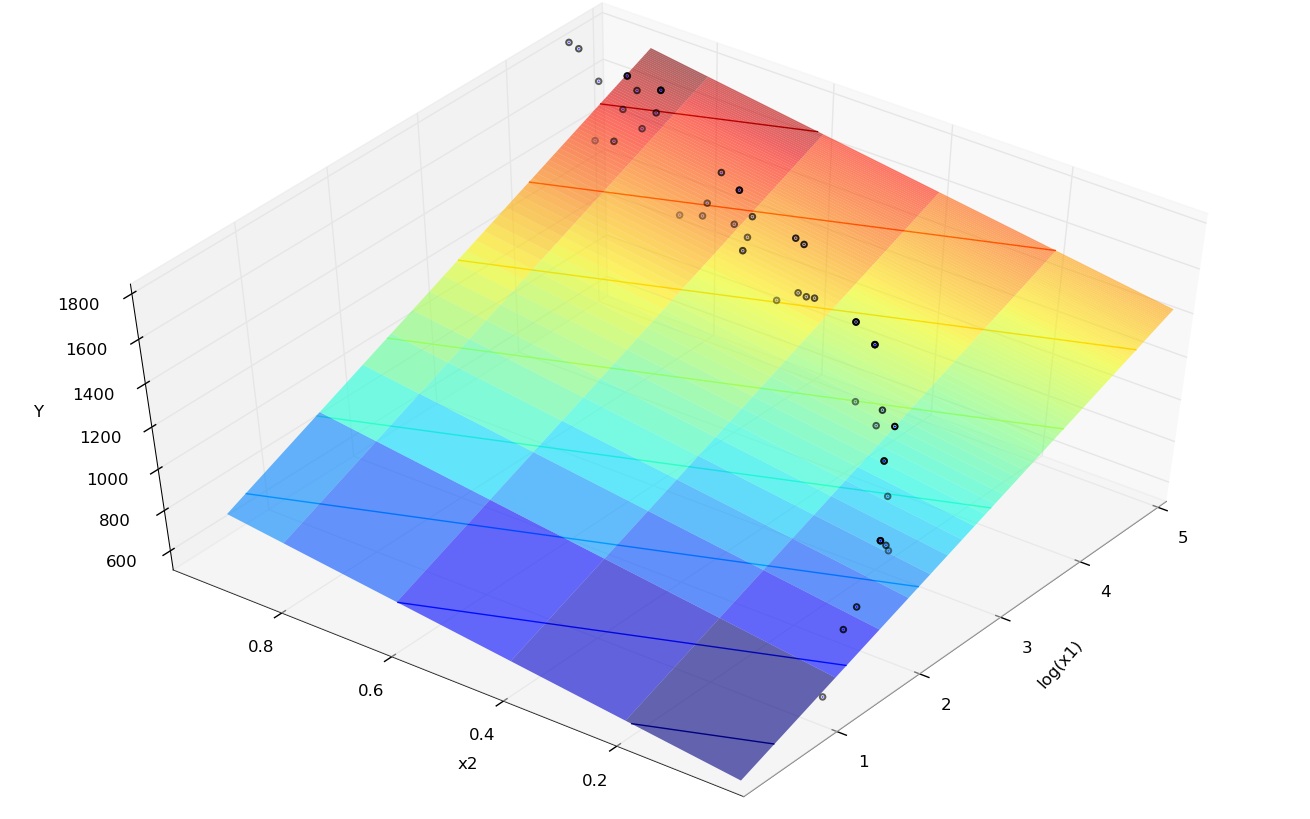
\includegraphics{image.jpg}
\end{center}
    \end{lstlisting}
  \end{block}
  \begin{block}{Flottant}
    Référencement par \lstinline|voir figure~\ref{fig:graphique}|
    \begin{lstlisting}
\usepackage{graphicx}
...
\begin{figure}[!ht]
  \centering
  \includegraphics{graph.png}
  \caption{Voici un beau graphique}
  \label{fig:graphique}
\end{figure}
    \end{lstlisting}
  \end{block}
  \begin{block}{Hybride: référençable mais non-flottant}
    Référencement par \lstinline|voir figure~\ref{fig:graphique}|
    \begin{lstlisting}
\usepackage{graphicx}
\usepackage{float}
...
\begin{figure}[H]
  ...
  \label{fig:graphique}
\end{figure}
    \end{lstlisting}
    ou
    \begin{lstlisting}
\usepackage{graphicx}
\usepackage{caption}
...
\begin{center}
  ...
  \captionof{figure}{Voici un beau graphique}
  \label{fig:graphique}
\end{center}
    \end{lstlisting}
  \end{block}
  \begin{block}{Scaling}
    \begin{lstlisting}
\usepackage{graphicx}
...
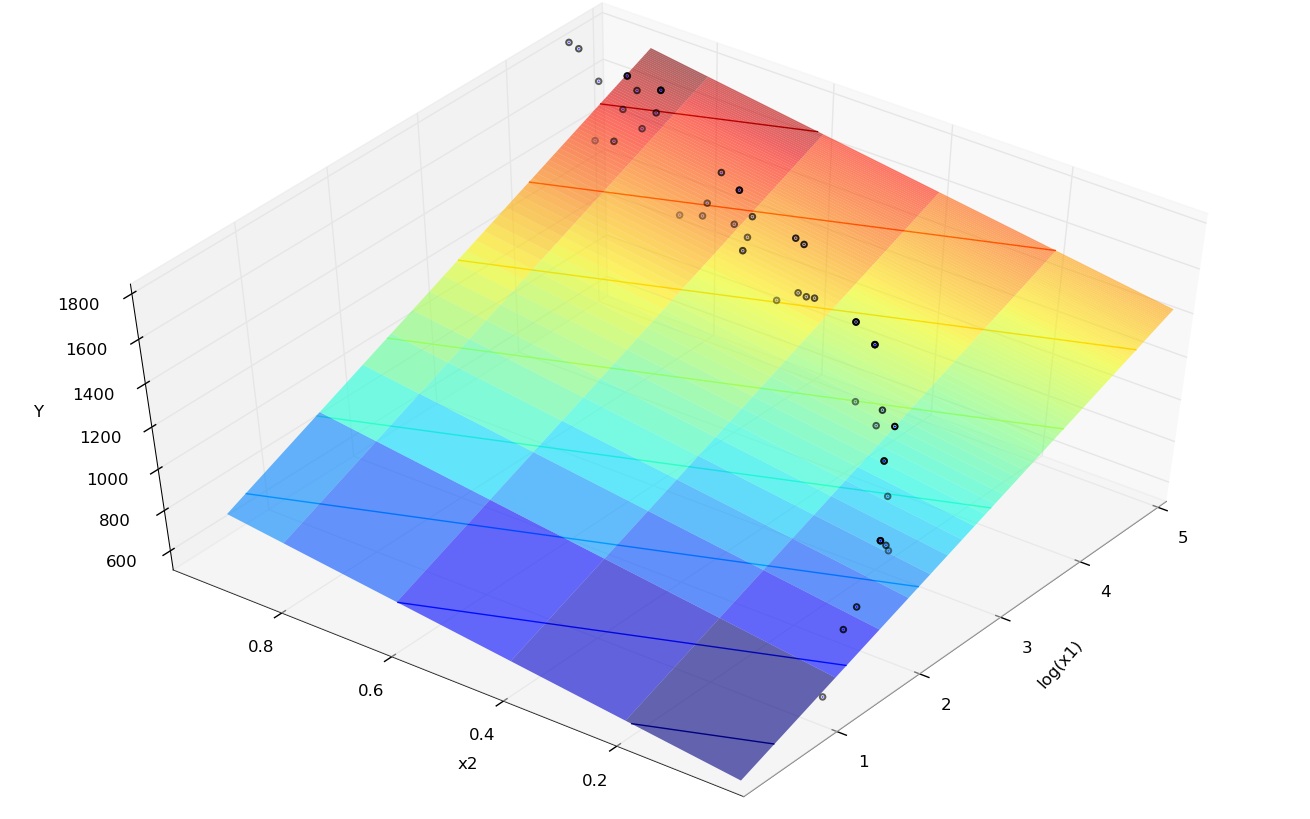
\includegraphics[width=\textwidth]{image.jpg} % Largeur d'une ligne de texte
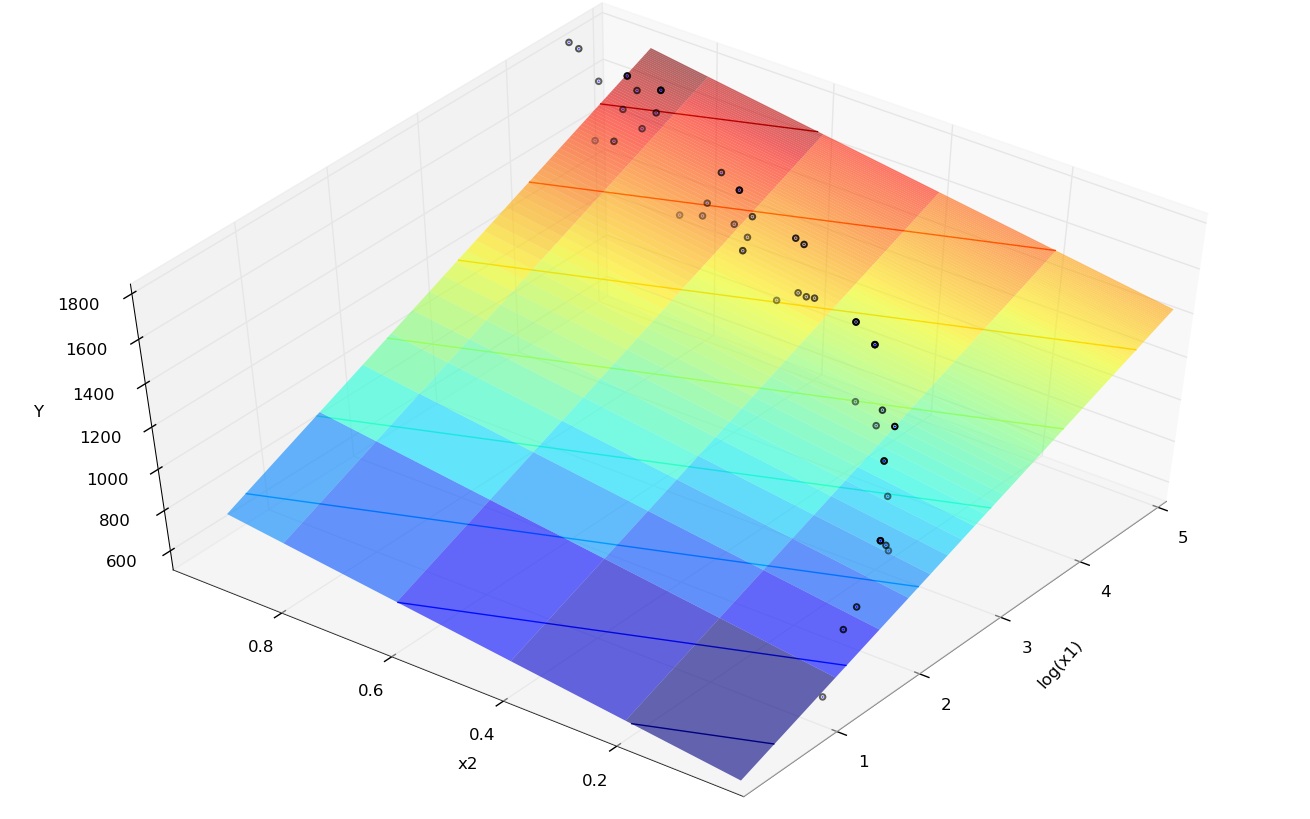
\includegraphics[height=4cm]{image.jpg} % Hauteur de 4cm
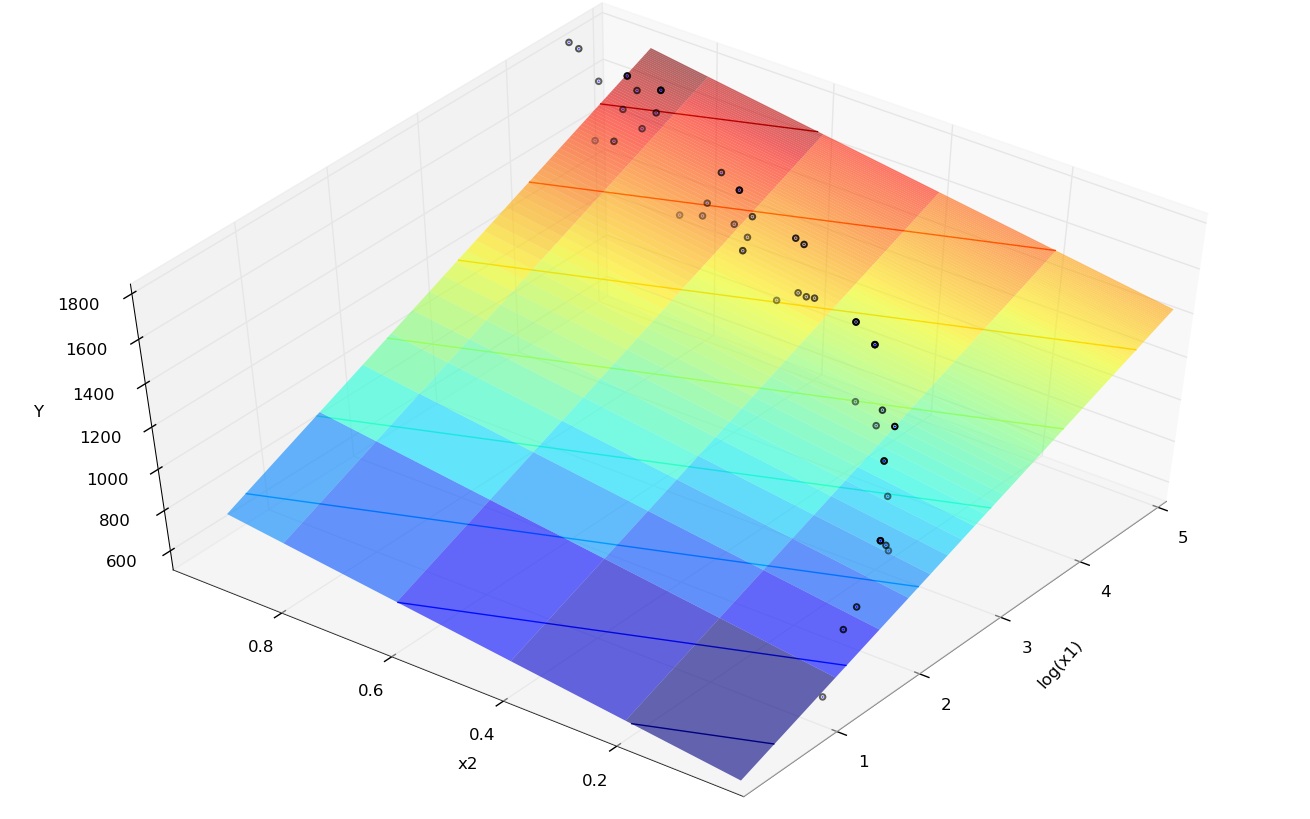
\includegraphics[scale=0.5]{image.png} % taille / 2
    \end{lstlisting}
  \end{block}

  \vspace{4.2em}

\begin{quote}
  1992: Extensive testing shows that 98.3\% of the time
  no matter which of the
  \lstinline|[h]|,
  \lstinline|[t]|,
  \lstinline|[b]|, or
  \lstinline|[p]|
  options is used,
  \LaTeX{} will put your \lstinline|table| at the end of the document.

  \vspace{1em}
  \hfill
  \em
  \begin{minipage}{8cm}
    DAVID F. GRIFFITHS and DESMOND J. HIGHAM, Great Moments in \LaTeX{} History (1997)
  \end{minipage}
\end{quote}

\end{frame}

\begin{frame}[fragile]{Exemple de figure}
	\fbox{
\includegraphics[width=\textwidth]{figure.jpg}}
\end{frame}

\begin{frame}[fragile]{Exemple de figure}
%\framesubtitle{Un contenant pour des éléments de type \textit{table} et \textit{figure}}

\begin{lstlisting}
\usepackage{graphicx}
...
Sur la figure~\ref{fig:ucl}, vous pouvez voir le logo UCL
mis a \SI{50}{\percent} de la largueur du texte.

\begin{figure}[!ht]
    \centering
        
\includegraphics[width=0.50\textwidth]{logo-ucl.jpg}
    \caption{Voici le logo UCL}
    \label{fig:ucl}
\end{figure}
\end{lstlisting}

\end{frame}
%	\vspace{0.5cm}
%	\hspace{1cm} \verb|\begin{|{\usebeamercolor[fg]{example text} \verb|itemize|}\verb|} |\\
%	\hspace{2cm} \verb|\item Premier élément de la liste|\\
%	\hspace{2cm} \verb|\item Deuxième élément de la liste|\\
%	\hspace{1cm} \verb|\end{|{\usebeamercolor[fg]{example text} \verb|itemize|}\verb|} |\\
%	\vspace{0.5cm}

\subsection{Les tableaux}
\begin{frame}[fragile,allowframebreaks]
  \frametitle{Tableaux}
  \begin{block}{Non-flottant}
    Référencement par ``ci-dessous'', \dots
    \begin{lstlisting}
\begin{center}
  \begin{tabular}{...}
    ...
  \end{tabular}
\end{center}
    \end{lstlisting}
  \end{block}
  \begin{block}{Flottant}
    Référencement par \lstinline|voir tableau~\ref{tab:data}|
    \begin{lstlisting}
\begin{table}
  \centering
  \begin{tabular}{...}
    ...
  \end{tabular}
  \caption{Voici un beau tableau}
  \label{tab:data}
\end{table}
    \end{lstlisting}
  \end{block}
  \begin{block}{Code}
    \begin{lstlisting}
\begin{tabular}{|lcr|}
  \hline
  A & B & C\\
  \hline
  a & b & c\\
  $\alpha$ & $\beta$ & $\gamma$\\
  \hline
\end{tabular}
    \end{lstlisting}
  \end{block}
  \begin{block}{Rendu}
\begin{tabular}{|lcr|}
  \hline
  A & B & C\\
  \hline
  a & b & c\\
  $\alpha$ & $\beta$ & $\gamma$\\
  \hline
\end{tabular}
  \end{block}
\end{frame}



\begin{frame}[fragile]{Exemple de tableau}
\begin{footnotesize}
\begin{lstlisting}
\begin{table}[!ht]
    \begin{center}
            \begin {tabular}{|l||c|} %% 2 columns
            \hline
                \textit{Inventaire} & \textbf{Nombre} \\
            \hline
                Chemises  & 4   \\
                Pulls     & 12  \\
                Pantalons & 1   \\
            \hline
            \end{tabular}
        \caption{Tableau relatif a l'inventaire}
    \end{center}
\end{table}
\end{lstlisting}
\end{footnotesize}
\begin{center}
\fbox{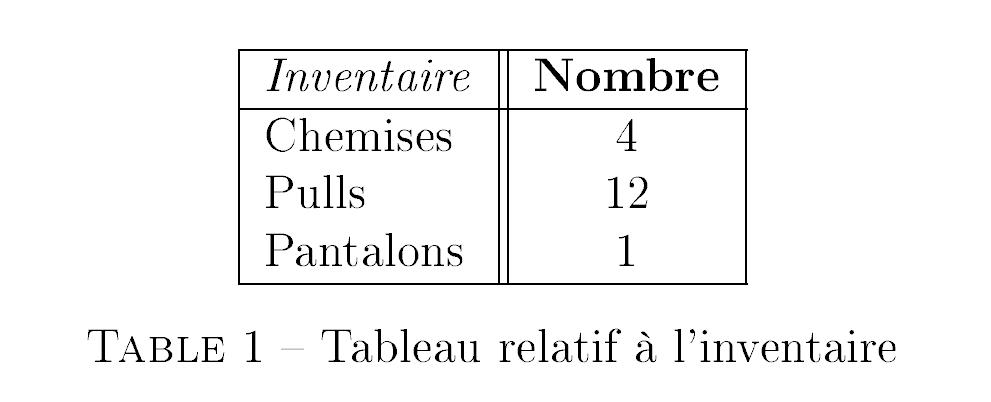
\includegraphics[width=0.6\textwidth]{table.jpg}}
\end{center}
\end{frame}
%-----------------------
\section{Sciences}
\subsection{Écrire des mathématiques}
\begin{frame}[fragile]{L'environnement mathématique}
\framesubtitle{Inclure des formules dans le texte}
On peut ajouter une formule mathématique dans du texte entre deux symboles \textbf{\$}.

\vspace{1cm}
\begin{center}
    \Large
  \begin{tabular}{lll}
    \verb|$x^{2n}$| & $\rightarrow$ &  $x^{2n}$\\
    \medskip
    \verb|$\sin(x)$| & $\rightarrow$ &  $\sin(x)$\\
  \end{tabular}
\end{center}
\end{frame}
\begin{frame}[fragile]{L'environnement mathématique}
\framesubtitle{Inclure des formules centrées hors du texte}
On peut aussi ajouter une formule mathématique centrées hors du texte entre deux symboles \textbf{\$\$}. Exemple:

\begin{columns}
  \begin{column}{0.45\textwidth}
    $|x|$ is positive for any value of $x$,
    we can define it like so
    $$x =
    \begin{cases}
      -x & \text{si }x < 0\\
      x & \text{sinon}.
    \end{cases}$$

    Be aware that
    $$|x + y| \neq |x| + |y|.$$
    However, we have the triangle inequality
    $$|x + y| \leq |x| + |y|$$
    for any $x,y \in \mathbb{C}$.
  \end{column}
  \begin{column}{0.45\textwidth}
    \begin{lstlisting}
\usepackage{amsmath} % for \begin{cases}
\usepackage{amssymb} % for \mathbb
...
$|x|$ is positive for
any value of $x$,
we can define it like so
$$x =
\begin{cases}
  -x & \text{si }x < 0\\
  x & \text{sinon}.
\end{cases}$$

Be aware that
$$|x + y| \neq |x| + |y|.$$
However, we have the triangle inequality
$$|x + y| \leq |x| + |y|$$
for any $x,y \in \mathbb{C}$.
    \end{lstlisting}
  \end{column}
\end{columns}
\end{frame}

\begin{frame}[fragile]{L'environnement mathématique}
\framesubtitle{Inclure des formules centrées hors du texte}
On peut aussi ajouter une formule mathématique centrées hors du texte entre deux symboles \textbf{\$\$}. Exemple:

\begin{columns}
  \begin{column}{0.45\textwidth}
    $|x|$ is positive for any value of $x$,
    we can define it like so
    $$x =
    \begin{cases}
      -x & \text{si }x < 0\\
      x & \text{sinon}.
    \end{cases}$$

    Be aware that
    $$|x + y| \neq |x| + |y|.$$
    However, we have the triangle inequality
    $$|x + y| \leq |x| + |y|$$
    for any $x,y \in \mathbb{C}$.
  \end{column}
  \begin{column}{0.45\textwidth}
    \begin{lstlisting}
\usepackage{amssymb} % for \mathbb
...
$|x|$ is positive for
any value of $x$,
we can define it like so
$$x =
\begin{cases}
  -x & \text{si }x < 0\\
  x & \text{sinon}.
\end{cases}$$

Be aware that
$$|x + y| \neq |x| + |y|.$$
However, we have the triangle inequality
$$|x + y| \leq |x| + |y|$$
for any $x,y \in \mathbb{C}$.
    \end{lstlisting}
  \end{column}
\end{columns}

\end{frame}



\begin{frame}[fragile]{L'environnement mathématique}
\framesubtitle{Formules numérotées}

Un environnement équation est prévu pour des formules plus longues, elles seront automatiquement centrées et numérotées pour être référencées

\begin{columns}
  \begin{column}{0.6\textwidth}
I like trains and the equation~\eqref{eq:euler}
\begin{align}
  \label{eq:euler}
  e^{i\pi} + 1 & = 0\\
  \notag
  p(x) & = \frac{1}{\sigma \sqrt{2\pi}}
  \exp
    \left(-\frac{(x-\mu)^2}
                {2\sigma^2}\right).
\end{align}
I also know that
\begin{align*}
  1 + 1 & = 2 & 1 + 2 & = 3\\
  2 + 3 & = 5 & 3 + 5 & = 8.
\end{align*}
  \end{column}
  \begin{column}{0.4\textwidth}
    \begin{lstlisting}
\usepackage{amsmath} % for eqref
...
I like trains and
the equation~\eqref{eq:euler}
\begin{align}
  \label{eq:euler}
  e^{i\pi} + 1 & = 0\\
  \notag
  p(x) & = \frac{1}{\sigma \sqrt{2\pi}}
  \exp
    \left(-\frac{(x-\mu)^2}
    {2\sigma^2}\right).
\end{align}
I also know that
\begin{align*}
  1 + 1 & = 2 & 1 + 2 & = 3\\
  2 + 3 & = 5 & 3 + 5 & = 8.
\end{align*}
    \end{lstlisting}
  \end{column}
\end{columns}

\end{frame}

\begin{frame}[fragile]{L'environnement mathématique}
\framesubtitle{Variable à plusieurs lettres}

Attention aux yeux du lecteurs (surtout ceux ayant un compas à portée de main).
$cube = c \cdot u \cdot b \cdot e = c \times u \times b \times e$.
Les variables plusieurs lettres doivent être différenciées de celles à une seule lettre.

%\begin{columns}
%  \begin{column}{0.6\textwidth}
\begin{center}
  \begin{tabular}{|c|c|}
    \hline
    Bad & Good\\
    \hline
    $cube(x) = x^3$ & $\mathsf{cube}(x) = x^3$\\
    \hline
    $flux_{in}(k_{orig}) = flux_{out}(k_{dest})$ & $\mathsf{flux}_{\text{in}}(k_{\text{orig}}) = \mathsf{flux}_{\text{out}}(k_{\text{dest}})$\\
    \hline
  \end{tabular}
\end{center}
%  \end{column}
%  \begin{column}{0.4\textwidth}
\begin{lstlisting}
\begin{center}
  \begin{tabular}{|c|c|}
    \hline
    Bad & Good\\
    \hline
    $cube(x) = x^3$ & $\mathsf{cube}(x) = x^3$\\
    \hline
    $flux_{in}(k_{orig}) = flux_{out}(k_{dest})$ & $\mathsf{flux}_{\text{in}}(k_{\text{orig}}) = \mathsf{flux}_{\text{out}}(k_{\text{dest}})$\\
    \hline
  \end{tabular}
\end{center}
\end{lstlisting}
%  \end{column}
%\end{columns}
\textbf{Problème} Le code se ralonge (solution dans quelques slides).
\end{frame}

\begin{frame}[fragile]{L'environnement mathématique}
\framesubtitle{Les classes}
Les espaces du code sont ignorés en math mode.
Comment \TeX détermine l'espacement à faire ?

Il distingue 8 classes.
Chaque symbole, caractère ou sous-formule est dans une classe qui détermine l'espacement autour de lui.
\begin{center}
  \begin{tabular}{cp{0.5\textwidth}l}
    Ordinary & \lstinline|/|, sous-formule (en général) & \lstinline|\mathord| or \lstinline|{}|\\
    Large operator & \lstinline|\sum|, \lstinline|\prod| & \lstinline|\mathop|\\
    Binary operation & \lstinline|+| & \lstinline|\mathbin|\\
    Relation & \lstinline|=|, \lstinline|:| & \lstinline|\mathrel|\\
    Opening & \lstinline|(| & \lstinline|\mathopen|\\
    Closing & \lstinline|)| & \lstinline|\mathclose|\\
    Punctuation & \lstinline|,| & \lstinline|\mathpunct|\\
    Variable family & \lstinline|x| & \\
    Interne & aucun symbole seul. Sous-formule avec fraction ou \lstinline|\left..\right| & \lstinline|\mathinner|\\
  \end{tabular}
\end{center}
\end{frame}


\begin{frame}[fragile]{L'environnement mathématique}
\framesubtitle{Large Operators}
Ces opérateurs mathématiques sont $\lim, \min, \max, \sum, \prod, \ldots$.
Quelle différence ? Leurs indices et exposant sont au dessus et en dessous et pas à leur droite.

\begin{columns}
  \begin{column}{0.6\textwidth}
\begin{align*}
  \min_{x \in \mathbb{R}^n} \|x\|\\
  \sum_{i = 1}^n x_i & = 1
\end{align*}

$\min_{x \in \mathbb{R}^n} \|x\|$ tel que $\sum_{i = 1}^n x_i = 1$.

$\min\limits_{x \in \mathbb{R}^n} \|x\|$ tel que $\sum\limits_{i = 1}^n x_i = 1$.
  \end{column}
  \begin{column}{0.4\textwidth}
\begin{lstlisting}
\begin{align*}
  \min_{x \in \mathbb{R}^n} \|x\|\\
  \sum_{i = 1}^n x_i & = 1
\end{align*}

$\min_{x \in \mathbb{R}^n} \|x\|$ tel que $\sum_{i = 1}^n x_i = 1$.

$\min\limits_{x \in \mathbb{R}^n} \|x\|$ tel que $\sum\limits_{i = 1}^n x_i = 1$.
\end{lstlisting}
  \end{column}
\end{columns}
\end{frame}

\begin{frame}[fragile]{L'environnement mathématique}
\framesubtitle{Binary Operations and Relations}
Tableau pris de ``Handbook of Writing for the Mathematical Sciences'', Nicholas J. Higham.
\begin{tabular}{cc|cc}
  Relation or Binary operation & Exemple & Ordinary symbol & Exemple\\
  \hline
  \lstinline|:| & $\{\,z : |z| \leq 1\,\}$ & \lstinline|\colon| & $f \colon A \to B$\\
  \lstinline|\mid| & $\{\,x \mid x > 0\,\}$ & \lstinline|\vert| ou \lstinline$|$ & $|z|$\\
  \lstinline|\setminus| & $\mathbb{R} \setminus \{0\}$ & \lstinline|\backslash| & $p \backslash n$\\
  \lstinline|\parallel| & $\vec{u} \parallel \vec{v}$ & \lstinline|\Vert| ou \lstinline$\|$ & $\|A\|$\\
  \lstinline|\perp| & $\vec{u} \perp \vec{v}$ & \lstinline|\bot| & $x_\bot$\\
  \lstinline|\in| & $x \in \mathbb{R}$ & $\epsilon$ & $\epsilon > 0$\\
\end{tabular}

\end{frame}


\begin{frame}[fragile]{L'environnement mathématique}
\framesubtitle{Définition de commandes, plus d'excuse !}

\begin{lstlisting}
\newcommand{\fin}{\mathsf{flux}_{\text{in}}}
\newcommand{\fout}{\mathsf{flux}_{\text{out}}}
% if \kor already exists
\renewcommand{\kor}{k_{\text{orig}}}
\newcommand{\kde}{k_{\text{dest}}}
\DeclareMathOperator{\pot}{potato} % mieux que \newcommand{\mathop{\mathrm{..}}}
% \min already exists: Trick for ``reDeclareMathOperator''
\let\min\relax% Set equal to \relax so that LaTeX thinks it's not defined
\DeclareMathOperator{\min}{minimum}
\newcommand{\badet}{et}
\newcommand{\goodet}{\mathbin{\mathrm{et}}}
\end{lstlisting}
\begin{columns}
  \begin{column}{0.45\textwidth}
    \begin{lstlisting}
\[ \alpha >> \beta \badet <x,y> = 0 => \]
    \end{lstlisting}
  \end{column}
  \begin{column}{0.35\textwidth}
    \[ \alpha >> \beta \badet <x,y> = 0 => \]
  \end{column}
  \begin{column}{0.2\textwidth}
    
\includegraphics[height=3em]{i_dont_want_to_live_on_this_planet_anymore.jpg}
  \end{column}
\end{columns}
\begin{columns}
  \begin{column}{0.45\textwidth}
    \begin{lstlisting}
\[ \alpha \gg \beta \goodet \langle x,y \rangle = 0 \Rightarrow \]
    \end{lstlisting}
  \end{column}
  \begin{column}{0.35\textwidth}
    \[ \alpha \gg \beta \goodet \langle x,y \rangle = 0 \Rightarrow \]
  \end{column}
  \begin{column}{0.2\textwidth}
    
\includegraphics[height=3em]{success_kid.jpg}
  \end{column}
\end{columns}
\end{frame}

\begin{frame}[fragile]{L'environnement mathématique}
\framesubtitle{Forcer un espacement}
Rarement utile !

\begin{center}
  \begin{tabular}{ll}
    Commande & espacements en mu (espace normal${}={}$6mu)\\
    \hline
    \lstinline|\!|     & $-$3\\
    \lstinline|\,|     &  3\\
    \lstinline|\:|     &  4\\
    \lstinline|\;|     &  5\\
    \lstinline|\ |     &  6\\
    \lstinline|\quad|  & 18\\
    \lstinline|\qquad| & 36
  \end{tabular}
\end{center}
\end{frame}

\begin{frame}[fragile]{L'environnement mathématique}
\framesubtitle{Forcer un espacement : Exemples}
\begin{columns}
  \begin{column}{0.5\textwidth}
    \begin{lstlisting}
\begin{align*}
  a & = u + v + w + x + y\\
    & \quad + z
\end{align*}
    \end{lstlisting}
  \end{column}
  \begin{column}{0.5\textwidth}
\begin{align*}
  a & = u + v + w + x + y\\
    & \quad + z
\end{align*}
  \end{column}
\end{columns}

Erreur courante: les ensembles besoin d'espacement (i.e. \lstinline|\,|) en compréhension mais pas en extension.
\begin{columns}
  \begin{column}{0.5\textwidth}
    \begin{lstlisting}
\begin{align*}
  \mathbb{R}_+ & = \{\, x \in \mathbb{R} \mid R \geq 0 \,\}\\
  \mathbb{R}_+ & = \{\, x \in \mathbb{R} : R \geq 0 \,\}\\
  \mathbb{N} & = \{0, 1, 2, 3, 4, \ldots\}\\
\end{align*}
    \end{lstlisting}
  \end{column}
  \begin{column}{0.5\textwidth}
\begin{align*}
  \mathbb{R}_+ & = \{\, x \in \mathbb{R} \mid R \geq 0 \,\}\\
  \mathbb{R}_+ & = \{\, x \in \mathbb{R} : R \geq 0 \,\}\\
  \mathbb{N} & = \{0, 1, 2, 3, 4, \ldots\}\\
\end{align*}
  \end{column}
\end{columns}
\end{frame}

\subsection{La physique}
\begin{frame}[fragile]
  \frametitle{Les unités}
  \lstinline|\usepackage{siunitx}|
  \begin{center}
    \begin{tabular}{ll}
      \num{314e-2} & \lstinline|\num{314e-2}|\\
      \ang{42} & \lstinline|\ang{42}|\\
      \si{g_{polymer}~mol_{cat}.s^{-1}} &
      \lstinline|\si{g_{polymer}~mol_{cat}.s^{-1}}|\\
      \si{\square\volt\cubic\lumen\per\farad} &
      \lstinline|\si{\square\volt\cubic\lumen\per\farad}|\\
      \SI{e-6}{\meter\per\second\per\ohm} &
      \lstinline|\SI{e-6}{\meter\per\second\per\ohm}|\\
      \SI[per-mode=symbol]{5.3e9}{m\per s} &
      \lstinline|\SI[per-mode=symbol]{5.3e9}{m\per s}|\\
      \SI[per-mode=symbol]{5.3e9}{\meter\per\second\per\ohm} &
      \lstinline|\SI[per-mode=symbol]{5.3e9}{\meter\per\second\per\ohm}|\\
      \SI[per-mode=fraction]{5e6}{\joule\per\second} &
      \lstinline|\SI[per-mode=fraction]{5e6}{\joule\per\second}|\\
      \SI{-273.15}{\celsius} &
      \lstinline|\SI{-273.15}{\celsius}|
    \end{tabular}
  \end{center}
  Super doc sur \url{http://ctan.org/pkg/siunitx}
\end{frame}

\subsection{La chimie}
\begin{frame}[fragile]
  \centering
  \frametitle{La chimie}
  \begin{lstlisting}
\usepackage{chemfig}
...
\chemfig{*6(-=(-CH_2OH)-(-COOH)=-=)}
  \end{lstlisting}
  \begin{center}
    \chemfig{*6(-=(-CH_2OH)-(-COOH)=-=)}
  \end{center}
  \begin{lstlisting}
\usepackage[version=3]{mhchem}
...
$$\ce{3H2O + 1/2H2O -> AgCl2- + H2_{(aq)}}$$
  \end{lstlisting}
  $$\ce{3H2O + 1/2H2O -> AgCl2- + H2_{(aq)}}$$
\end{frame}

\subsection{Les circuits}
\begin{frame}[fragile]
  \begin{lstlisting}
    \usepackage{circuitikz}
    ...
    \begin{circuitikz}
      \draw (0,0) to [sI, v=$V_2$] (0,-3);
      \draw (6,-3) to[short, i = $I_2$] (0,-3);
      \draw (0,0) to [R = R, v = $V_R$] (3,0);
      \draw (3,0) to [L = L, v = $V_L$] (6,0);
      \draw (6,0) to [C = C, v = $V_C$] (6,-3);
    \end{circuitikz}
  \end{lstlisting}
  \begin{center}
    \begin{circuitikz}
      \draw (0,0) to [sI, v=$V_2$] (0,-3);
      \draw (6,-3) to[short, i = $I_2$] (0,-3);
      \draw (0,0) to [R = R, v = $V_R$] (3,0);
      \draw (3,0) to [L = L, v = $V_L$] (6,0);
      \draw (6,0) to [C = C, v = $V_C$] (6,-3);
    \end{circuitikz}
  \end{center}
\end{frame}

%%%%%%%%%%%%%

\section{Références}

\subsection{Références des éléments du texte}
\begin{frame}[fragile]
\frametitle{\insertsubsection}
\begin{itemize}
  \item Facile de faire référence à un numéro et la page d'une section et d'un environnement (\texttt{figure}, \texttt{equation}, \texttt{table}).
  \item D'un coté une étiquette :
    \begin{itemize}
      \item \lstinline|\label{id}|.
    \end{itemize}
  \item De l'autre une référence à cette étiquette :
    \begin{itemize}
      \item \lstinline|\ref{id}|
      \item \lstinline|\pageref{id}|
      \item \lstinline|\vpageref{id}| du paquet \lstinline|varioref|
    \end{itemize}
\end{itemize}
\begin{columns}
  \begin{column}{0.5\textwidth}
    \label{id}
    Nous sommes section~\ref{id},
    page~\pageref{id},
    \vpageref{id}.
  \end{column}
  \begin{column}{0.5\textwidth}
    \begin{lstlisting}
\label{ref}
Nous sommes section~\ref{ref},
page~\pageref{ref},
\vpageref{ref}.
    \end{lstlisting}
  \end{column}
\end{columns}

\end{frame}

\subsection{Footnote}
\begin{frame}[fragile]
  \frametitle{Footnote}
  \begin{lstlisting}
    The earth\footnote{mostly harmless} was destroyed
    by Vogons\footnote{They have the worst poetry in the universe}.

    But Don't Panic\footnote{By the way, the answer is 42},
    even when you're at the restaurant at
    the end of the universe.
  \end{lstlisting}
  \begin{block}{Result}
    The earth\footnote{Mostly harmless} was destroyed
    by Vogons\footnote{They have the worst poetry in the universe}.

    But Don't Panic\footnote{By the way, the answer is 42},
    even when you're at the restaurant at
    the end of the universe.
  \end{block}
\end{frame}

\subsection{Bibliographie}
\begin{frame}
\frametitle{\insertsubsection}
Deux possibilités pour maintenir une bibliographie:
\begin{itemize}
\item Éditer une bibliographie à la main (s'il y a très peu de référence, voir exemple)
\item Les fichiers \texttt{bib}
	\begin{itemize}
		\item Disponible avec les revues scientifiques et Google Scholar
		\item En utilisant le plugin \href{https://www.zotero.org/}{Zotero} pour récupérer les informations d'un \href{http://www.amazon.fr/LaTeX-HowTo-S\%C3\%A9bastien-Comb\%C3\%A9fis/dp/1446708314/ref=sr_1_5?ie=UTF8&qid=1363022579&sr=8-5}{site}
	\end{itemize}
\item Pour les utiliser
	\begin{itemize}
		\item Ajouter la source dans le fichier \texttt{bib}.
		\item ``Compiler'' le fichier Bib\TeX{} puis ``recompiler'' le document.
		\item Inclure dans son texte la commande \texttt{cite} avec l'étiquette de la source à référencer.
		\item \LaTeX{} inclut la référence dans le texte et ajoute la source à la bibliographie.
	\end{itemize}
\end{itemize}
\end{frame}

\begin{frame}[fragile,allowframebreaks]
  \frametitle{Bibliography}
  \begin{columns}
    \begin{column}{0.45\textwidth}
  \begin{block}{Citer}
    \begin{lstlisting}
\cite{goossens93}
\cite[p.~42]{goossens93}
\cite{goossens93,combefis11,...}
    \end{lstlisting}
  \end{block}
  \begin{block}{Inclure la bibliographie}
    \begin{lstlisting}
\bibliographystyle{plain}
\bibliography{biblio}
    \end{lstlisting}
  \end{block}
\end{column}
\begin{column}{0.45\textwidth}
  \centering
  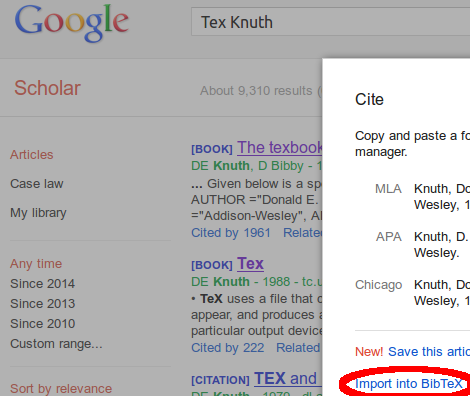
\includegraphics[width=\textwidth]{img/scholar_circle.png}
\end{column}
\end{columns}

\begin{description}
  \item[bad] \lstinline|voir\cite{goossens93}|
  \item[ok] \lstinline|voir \cite{goossens93}|
  \item[ok] \lstinline|voir~\cite{goossens93}|
\end{description}

\bibliographystyle{plain}
  \begin{block}{Élément d'une bibliographie}
    À mettre dans \lstinline|biblio.bib|
    \begin{lstlisting}
@book{goossens93,
    author    = "Michel Goossens and Frank Mittelbach and Alexander Samarin",
    title     = "The LaTeX Companion",
    year      = "1993",
    publisher = "Addison-Wesley",
    address   = "Reading, Massachusetts"
}
@book{knuth1986texbook,
  title={The texbook},
  author={Knuth, Donald Ervin and Bibby, Duane},
  volume={1993},
  year={1986},
  publisher={Addison-Wesley Reading, MA, USA}
}
    \end{lstlisting}
  \end{block}
\end{frame}


\subsection{include et input}
\begin{frame}[fragile]
  \frametitle{include et input}
  \begin{columns}
    \begin{column}{0.5\textwidth}
      Simple ``copier/coller''.
      \begin{lstlisting}
\input{chap1}
\input{chap2}
\input{chap3}
\input{chap4}
      \end{lstlisting}
    \end{column}
    \begin{column}{0.5\textwidth}
      \lstinline|\include{x}| c'est comme faire
      \begin{lstlisting}
\clearpage
\input{x}
\clearpage
      \end{lstlisting}
      Il y a aussi \lstinline|includeonly| pour gagner du temps
      \begin{lstlisting}
\includeonly{chap1,chap3}
...
\include{chap1}
\include{chap2}
\include{chap3}
\include{chap4}
      \end{lstlisting}
    \end{column}
  \end{columns}
\end{frame}

\AtBeginSection[]{} %% stop TOC

\section{Exercices}
\begin{frame}
\frametitle{Exerçons-nous}
	\begin{itemize}
		\item<1-> Télécharger le document \textbf{exemple.pdf}
		\item<2-> Reproduire une structure similaire :
			\begin{itemize}
				\item page de titre
				\item table des matières
				\item liste, tableau, figure
				\item math en ligne, hors-ligne
				\item références
				\item \dots
			\end{itemize}
		\item<3-> Chercher de l'information :
			\begin{itemize}
				\item \url{http://en.wikibooks.org/wiki/LaTeX}
				\item \url{http://www.grappa.univ-lille3.fr/FAQ-LaTeX}
                \item \url{http://www.andy-roberts.net/writing/latex}
                \item \url{http://ctan.org/pkg/packagename} ou \lstinline[language=sh,morekeywords={texdoc}]{$ texdoc packagename}
				\item Google est ton ami !
                \item \url{http://www.sharelatex.com/learn}
                \item La version de StackExchange spécialisée pour le \TeX:
      \url{tex.stackexchange.com}.
				\item Livres:
				\begin{itemize}
					\item \LaTeX HowTo par Sébastien Combéfis (EN/FR)
					\item Framabook \LaTeX
				\end{itemize}
				\item \url{http://www.tablesgenerator.com/}
			\end{itemize}
	\end{itemize}
\end{frame}


\end{document}
